%%%%%%%%%%%%%%%%%%%%%%%%%%%%%%%%%%%%%%%%%%%%%%%%%%%%%%%%%%%%%%%%%%%%%%%%%%%%%%%%%
% Template: Exam
%
% Por: Abrantes Araújo Silva Filho
%      abrantesasf@gmail.com
%
% Citação: Se você gostou deste template, por favor ajude a divulgá-lo mantendo
%          o link para meu repositório GitHub em:
%          https://github.com/abrantesasf/LaTeX
%%%%%%%%%%%%%%%%%%%%%%%%%%%%%%%%%%%%%%%%%%%%%%%%%%%%%%%%%%%%%%%%%%%%%%%%%%%%%%%%%




%%%%%%%%%%%%%%%%%%%%%%%%%%%%%%%%%%%%%%%%%%%%%%%%%%%%%%%%%%%%%%%%%%%%%%%%%%%%%%%%%
%%% Configura o tipo de documento, papel, tamanho da fonte e informações básicas
%%% para as proriedades do PDF/DVIPS e outras propriedades do documento
\RequirePackage{ifpdf}
\ifpdf
  % Classe, língua e tamanho da fonte padrão. Outras opções a considerar:
  %   draft
  %   onecolumn (padrão) ou twocolumn (OU usar o package multicol)
  %   fleqn com ou sem leqno (alinhamento à esquerda das fórmulas e dos números)
  %   oneside (padrão para article ou report) ou twoside (padrão para book)
  %   answers = imprime respostas para o gabarito
  \documentclass[pdftex, brazil, 12pt, oneside, addpoints]{exam}
\else
  % Classe, língua e tamanho da fonte padrão. Outras opções a considerar:
  %   draft
  %   onecolumn (padrão) ou twocolumn (OU usar o package multicol)
  %   fleqn com ou sem leqno (alinhamento à esquerda das fórmulas e dos números)
  %   oneside (padrão para article ou report) ou twoside (padrão para book)
  %   answers = imprime respostas para o gabarito
  \documentclass[brazil, 12pt, oneside, addpoints]{exam}
\fi


%%%%%%%%%%%%%%%%%%%%%%%%%%%%%%%%%%%%%%%%%%%%%%%%%%%%%%%%%%%%%%%%%%%%%%%%%%%%%%%%%
%%% Carrega pacotes iniciais necessários para estrutura de controle e para a
%%% criação e o parse de novos comandos
\usepackage{ifthen}
\usepackage{xparse}


%%%%%%%%%%%%%%%%%%%%%%%%%%%%%%%%%%%%%%%%%%%%%%%%%%%%%%%%%%%%%%%%%%%%%%%%%%%%%%%%%
%%% Configuração do tamanho da página, margens, espaçamento entrelinhas e, se
%%% necessário, ativa a indentação dos primeiros parágrafos.
\ifpdf
  \usepackage[pdftex]{geometry}
\else
  \usepackage[dvips]{geometry}
\fi
\geometry{a4paper, left=2.0cm, right=2.0cm, top=2.0cm, bottom=2.0cm}

\usepackage{setspace}
  \singlespacing
  %\onehalfspacing
  %\doublespacing


%%%%%%%%%%%%%%%%%%%%%%%%%%%%%%%%%%%%%%%%%%%%%%%%%%%%%%%%%%%%%%%%%%%%%%%%%%%%%%%%%
%%% Configurações de encoding, lingua e fontes:
\usepackage[T1]{fontenc}
\usepackage[utf8]{inputenc}
\usepackage{babel}

% Altera a fonte padrão do documento (nem todas funcionam em modo math):
%   phv = Helvetica
%   ptm = Times
%   ppl = Palatino
%   pbk = bookman
%   pag = AdobeAvantGarde
%   pnc = Adobe NewCenturySchoolBook
\renewcommand{\familydefault}{ppl}


%%%%%%%%%%%%%%%%%%%%%%%%%%%%%%%%%%%%%%%%%%%%%%%%%%%%%%%%%%%%%%%%%%%%%%%%%%%%%%%%%
%%% Configurações de cabeçalho e rodapé (não pode usar fancyhdr pois ocorre conflito):
\pagestyle{headandfoot}
\runningheadrule
\firstpageheader{}{}{}
\runningheader{Atividade de Recuperação da Aprendizagem}{}{Junho/2019}
\firstpagefooter{}{}{Página \thepage\ de \numpages}
\runningfooter{}{}{Página \thepage\ de \numpages}
\runningfootrule


%%%%%%%%%%%%%%%%%%%%%%%%%%%%%%%%%%%%%%%%%%%%%%%%%%%%%%%%%%%%%%%%%%%%%%%%%%%%%%%%%
%%% Carrega pacotes para referências cruzadas, citações dentro do documento,
%%% links para internet e outros.Configura algumas opções.
%%% Não altere a ordem de carregamento dos packages.
\usepackage{varioref}
\ifpdf
  \usepackage[pdftex]{hyperref}
    \hypersetup{
      % Informações variáveis em cada documento (MUDE AQUI!):
      pdftitle={Atividade de Recuperação da Aprendizagem},
      pdfauthor={Abrantes Araújo Silva Filho},
      pdfsubject={Sistemas de Equações Lineares},
      pdfkeywords={sistemas de equações lineares},
      pdfinfo={
        CreationDate={}, % Ex.: D:AAAAMMDDHH24MISS
        ModDate={}       % Ex.: D:AAAAMMDDHH24MISS
      },
      % Coisas que você não deve alterar se não souber o que está fazendo:
      unicode=true,
      pdflang={pt-BR},
      bookmarksopen=true,
      bookmarksnumbered=true,
      bookmarksopenlevel=5,
      pdfdisplaydoctitle=true,
      pdfpagemode=UseOutlines,
      pdfstartview=FitH,
      pdfcreator={LaTeX with hyperref package},
      pdfproducer={pdfTeX},
      pdfnewwindow=true,
      colorlinks=true,
      citecolor=green,
      linkcolor=red,
      filecolor=cyan,
      urlcolor=blue
    }
\else
  \usepackage{hyperref}
\fi
\usepackage{cleveref}
\usepackage{url}


%%%%%%%%%%%%%%%%%%%%%%%%%%%%%%%%%%%%%%%%%%%%%%%%%%%%%%%%%%%%%%%%%%%%%%%%%%%%%%%%%
%%% Carrega bibliotecas de símbolos (matemáticos, físicos, etc.), fontes
%%% adicionais, e configura algumas opções
\usepackage{amsmath}
\usepackage{amssymb}
\usepackage{amsfonts}
\usepackage{siunitx}
  \sisetup{group-separator = {.}}
  \sisetup{group-digits = {false}}
  \sisetup{output-decimal-marker = {,}}
\usepackage{bm}
\usepackage{cancel}
% Altera separador decimal via comando, se necessário (prefira o siunitx):
%\mathchardef\period=\mathcode`.
%\DeclareMathSymbol{.}{\mathord}{letters}{"3B}
\usepackage{esvect}
  

%%%%%%%%%%%%%%%%%%%%%%%%%%%%%%%%%%%%%%%%%%%%%%%%%%%%%%%%%%%%%%%%%%%%%%%%%%%%%%%%%
%%% Carrega packages relacionados à computação
\usepackage{algorithm2e}
\usepackage{algorithmicx}
\usepackage{algpseudocode}
\usepackage{listings}
  \lstset{literate=
    {á}{{\'a}}1 {é}{{\'e}}1 {í}{{\'i}}1 {ó}{{\'o}}1 {ú}{{\'u}}1
    {Á}{{\'A}}1 {É}{{\'E}}1 {Í}{{\'I}}1 {Ó}{{\'O}}1 {Ú}{{\'U}}1
    {à}{{\`a}}1 {è}{{\`e}}1 {ì}{{\`i}}1 {ò}{{\`o}}1 {ù}{{\`u}}1
    {À}{{\`A}}1 {È}{{\'E}}1 {Ì}{{\`I}}1 {Ò}{{\`O}}1 {Ù}{{\`U}}1
    {ä}{{\"a}}1 {ë}{{\"e}}1 {ï}{{\"i}}1 {ö}{{\"o}}1 {ü}{{\"u}}1
    {Ä}{{\"A}}1 {Ë}{{\"E}}1 {Ï}{{\"I}}1 {Ö}{{\"O}}1 {Ü}{{\"U}}1
    {â}{{\^a}}1 {ê}{{\^e}}1 {î}{{\^i}}1 {ô}{{\^o}}1 {û}{{\^u}}1
    {Â}{{\^A}}1 {Ê}{{\^E}}1 {Î}{{\^I}}1 {Ô}{{\^O}}1 {Û}{{\^U}}1
    {œ}{{\oe}}1 {Œ}{{\OE}}1 {æ}{{\ae}}1 {Æ}{{\AE}}1 {ß}{{\ss}}1
    {ű}{{\H{u}}}1 {Ű}{{\H{U}}}1 {ő}{{\H{o}}}1 {Ő}{{\H{O}}}1
    {ç}{{\c c}}1 {Ç}{{\c C}}1 {ø}{{\o}}1 {å}{{\r a}}1 {Å}{{\r A}}1
    {€}{{\euro}}1 {£}{{\pounds}}1 {«}{{\guillemotleft}}1
    {»}{{\guillemotright}}1 {ñ}{{\~n}}1 {Ñ}{{\~N}}1 {¿}{{?`}}1
  }
  

%%%%%%%%%%%%%%%%%%%%%%%%%%%%%%%%%%%%%%%%%%%%%%%%%%%%%%%%%%%%%%%%%%%%%%%%%%%%%%%%%
%%% Ativa suporte extendido a cores
\usepackage[svgnames]{xcolor} % Opções de cores: usenames (16), dvipsnames (64),
                              % svgnames (150) e x11names (300).


%%%%%%%%%%%%%%%%%%%%%%%%%%%%%%%%%%%%%%%%%%%%%%%%%%%%%%%%%%%%%%%%%%%%%%%%%%%%%%%%%
%%% Suporte à importação de gráficos externos
\ifpdf
  \usepackage[pdftex]{graphicx}
\else
  \usepackage[dvips]{graphicx}
\fi


%%%%%%%%%%%%%%%%%%%%%%%%%%%%%%%%%%%%%%%%%%%%%%%%%%%%%%%%%%%%%%%%%%%%%%%%%%%%%%%%%
%%% Suporte à criação de gráficos proceduralmente na LaTeX:
\usepackage{tikz}
  \usetikzlibrary{arrows,automata,backgrounds,matrix,patterns,positioning,shapes,shadows}


%%%%%%%%%%%%%%%%%%%%%%%%%%%%%%%%%%%%%%%%%%%%%%%%%%%%%%%%%%%%%%%%%%%%%%%%%%%%%%%%%
%%% Packages para tabelas
\usepackage{array}
\usepackage{longtable}
\usepackage{tabularx}
\usepackage{tabu}
\usepackage{lscape}
\usepackage{colortbl}  
\usepackage{booktabs}
\newcolumntype{M}[1]{>{\centering\arraybackslash}m{#1}}
%\newcolumntype{ML}[1]{>{$}l<{$}}
%\newcolumntype{MR}[1]{>{R}r<{R}}
\newcolumntype{L}[1]{>{\arraybackslash}m{#1}}
\newcolumntype{N}{@{}m{0pt}@{}}


%%%%%%%%%%%%%%%%%%%%%%%%%%%%%%%%%%%%%%%%%%%%%%%%%%%%%%%%%%%%%%%%%%%%%%%%%%%%%%%%%
%%% Packages ambientes de listas
\usepackage{enumitem}
\usepackage[ampersand]{easylist}


%%%%%%%%%%%%%%%%%%%%%%%%%%%%%%%%%%%%%%%%%%%%%%%%%%%%%%%%%%%%%%%%%%%%%%%%%%%%%%%%%
%%% Packages para suporte a ambientes floats, captions, etc.:
\usepackage{float}
\usepackage{wrapfig}
\usepackage{placeins}
\usepackage{caption}
\usepackage{sidecap}
\usepackage{subcaption}


%%%%%%%%%%%%%%%%%%%%%%%%%%%%%%%%%%%%%%%%%%%%%%%%%%%%%%%%%%%%%%%%%%%%%%%%%%%%%%%%%
%%% Meus comandos específicos:
% Commando para ``italizar´´ palavras em inglês (e outras línguas!):
\newcommand{\ingles}[1]{\textit{#1}}

% Commando para colocar o espaço correto entre um número e sua unidade:
\newcommand{\unidade}[2]{\ensuremath{#1\,\mathrm{#2}}}
\newcommand{\unidado}[2]{{#1}\,{#2}}

% Produz ordinal masculino ou feminino dependendo do segundo argumento:
\newcommand{\ordinal}[2]{%
#1%
\ifthenelse{\equal{a}{#2}}%
{\textordfeminine}%
{\textordmasculine}}


%%%%%%%%%%%%%%%%%%%%%%%%%%%%%%%%%%%%%%%%%%%%%%%%%%%%%%%%%%%%%%%%%%%%%%%%%%%%%%%%%
%%% Hifenização específica quando o LaTeX/Babel não conseguirem hifenizar:
\babelhyphenation{Git-Hub}


%%%%%%%%%%%%%%%%%%%%%%%%%%%%%%%%%%%%%%%%%%%%%%%%%%%%%%%%%%%%%%%%%%%%%%%%%%%%%%%%%
%%% Comandos específicos para a classe EXAM deste documento:
\newcommand{\umalinha}{\fillwithlines{0.25in}}
\newcommand{\duaslinhas}{\fillwithlines{0.50in}}
\newcommand{\treslinhas}{\fillwithlines{0.75in}}
\newcommand{\quatrolinhas}{\fillwithlines{1.00in}}
\newcommand{\cincolinhas}{\fillwithlines{1.25in}}
\newcommand{\seislinhas}{\fillwithlines{1.50in}}
\newcommand{\setelinhas}{\fillwithlines{1.75in}}
\newcommand{\oitolinhas}{\fillwithlines{2.00in}}
\newcommand{\novelinhas}{\fillwithlines{2.25in}}
\newcommand{\dezlinhas}{\fillwithlines{2.50in}}

% Verdadeiro ou Falvo para a classe EXAM
\newcommand{\vf}[1][{}]{%
  \fillin[#1][0.25in]%
}

% Título das respostas:
%\renewcommand{\solutiontitle}{\noindent\textbf{Resposta:}\par\noindent}
\renewcommand{\solutiontitle}{\noindent}
%\shadedsolutions
%\SolutionEmphasis{\itshape}

% Comandos para vetores
\newcommand{\vetor}[1]{\ensuremath{\vv{#1}}}
\newcommand{\vetori}{\ensuremath{\hat{i}}}
\newcommand{\vetorj}{\ensuremath{\hat{j}}}
\newcommand{\vetork}{\ensuremath{\hat{k}}}
\newcommand{\norma}[2]{\ensuremath{||\vetor{#2}||_{#1}}}


%%%%%%%%%%%%%%%%%%%%%%%%%%%%%%%%%%%%%%%%%%%%%%%%%%%%%%%%%%%%%%%%%%%%%%%%%%%%%%%%%
%%%%%%%%%%%%%%%%%%%%%%%%%%%%%%%%%%%%%%%%%%%%%%%%%%%%%%%%%%%%%%%%%%%%%%%%%%%%%%%%%
%%%%%%%%%%%%%%%%%%%%%%%%%%%%%%%%%%%%%%%%%%%%%%%%%%%%%%%%%%%%%%%%%%%%%%%%%%%%%%%%%
%%%%%%%%%%%%%%%%%%%%%%%%%%%%%%%%%%%%%%%%%%%%%%%%%%%%%%%%%%%%%%%%%%%%%%%%%%%%%%%%%
%%%%%%%%%%%%%%%%%%%%%%%%%%%%%% COMEÇA O DOCUMENTO %%%%%%%%%%%%%%%%%%%%%%%%%%%%%%%
%%%%%%%%%%%%%%%%%%%%%%%%%%%%%%%%%%%%%%%%%%%%%%%%%%%%%%%%%%%%%%%%%%%%%%%%%%%%%%%%%
%%%%%%%%%%%%%%%%%%%%%%%%%%%%%%%%%%%%%%%%%%%%%%%%%%%%%%%%%%%%%%%%%%%%%%%%%%%%%%%%%
%%%%%%%%%%%%%%%%%%%%%%%%%%%%%%%%%%%%%%%%%%%%%%%%%%%%%%%%%%%%%%%%%%%%%%%%%%%%%%%%%
%%%%%%%%%%%%%%%%%%%%%%%%%%%%%%%%%%%%%%%%%%%%%%%%%%%%%%%%%%%%%%%%%%%%%%%%%%%%%%%%%
\begin{document}


%%%%%%%%%%%%%%%%%%%%%%%%%%%%%%%%%%%%%%%%%%%%%%%%%%%%%%%%%%%%%%%%%%%%%%%%%%%%%%%%%
%%%%%%%%%%%%%%%%%%%%%%%%%%%%%%%%%%%%%%%%%%%%%%%%%%%%%%%%%%%%%%%%%%%%%%%%%%%%%%%%%
%%%%%%%%%%%%%%%%%%%%%%%%%%%%%%%%%%%%%%%%%%%%%%%%%%%%%%%%%%%%%%%%%%%%%%%%%%%%%%%%%
\begin{coverpages}

\begin{center}
\textbf{\textit{\Large%
Álgebra Linear e Geometria Analítica}}
\end{center}

\vspace{1cm}

\begin{figure}[H]
\begin{center}
\fbox{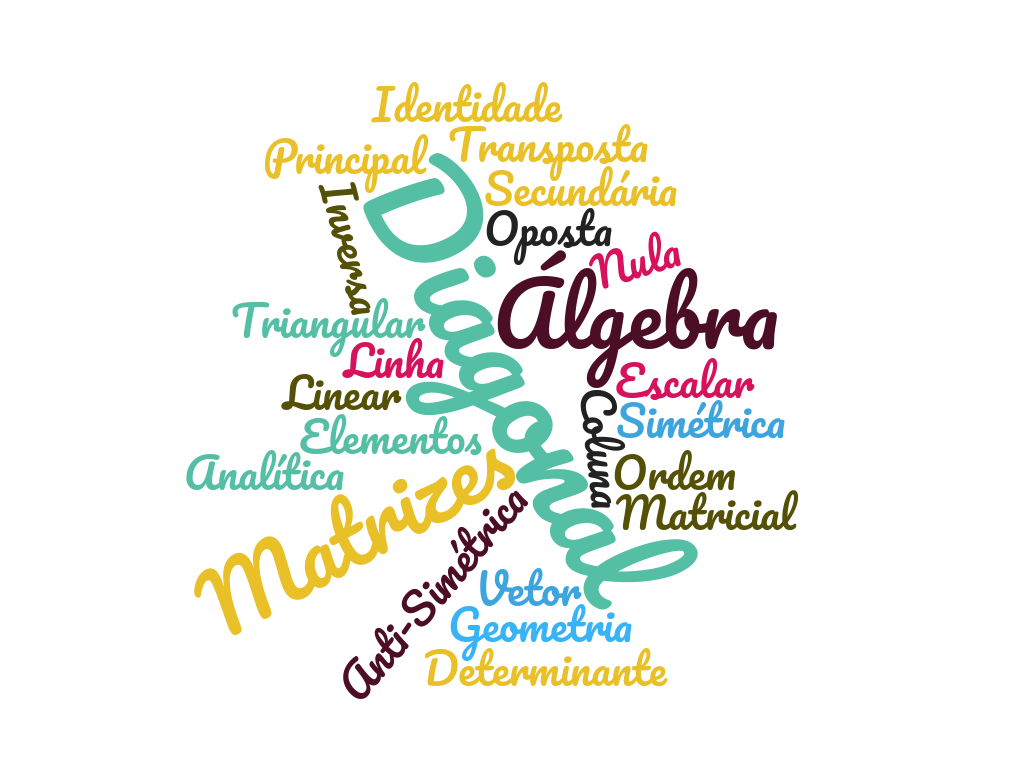
\includegraphics[scale=0.4]{linear_algebra.png}}
\end{center}
\end{figure}

\vspace{1cm}

\begin{center}
\textit{\textbf{\Large%
    --- Atividade de Recuperação da Aprendizagem ---\\%
\ \\%
    Sistemas de Equações Lineares\\%
\ \\%
Junho/2019}}
\end{center}

%\vspace{1cm}
%\begin{flushright}
%\textbf{Monitor(es):}\\
%\textit{Monitor 1\\
%Monitor 2}
%\end{flushright}

%\begin{center}
%  \fbox{\fbox{\parbox{5.5in}{\centering
%        Answer the questions in the spaces provided on the
%        question sheets. If you run out of room for an answer,
%        continue on the back of the page.}}}
%\end{center}

\end{coverpages}

\newpage


%%%%%%%%%%%%%%%%%%%%%%%%%%%%%%%%%%%%%%%%%%%%%%%%%%%%%%%%%%%%%%%%%%%%%%%%%%%%%%%%%
%%%%%%%%%%%%%%%%%%%%%%%%%%%%%%%%%%%%%%%%%%%%%%%%%%%%%%%%%%%%%%%%%%%%%%%%%%%%%%%%%
%%%%%%%%%%%%%%%%%%%%%%%%%%%%%%%%%%%%%%%%%%%%%%%%%%%%%%%%%%%%%%%%%%%%%%%%%%%%%%%%%
\makebox[15cm]{Nome:\enspace\hrulefill}

\vspace{0.5cm}

\makebox[15cm]{Curso:\enspace\hrulefill}

\fullwidth{\section{Instruções importantes}}

Esta \emph{Atividade de Recuperação da Aprendizagem} consiste de
11 questões que abordam o seguinte conteúdo:

\begin{itemize}
\item Sistemas de Equações Lineares:
  \begin{itemize}
  \item Reconhecimento de equações lineares
  \item Classificação de sistemas lineares
  \item Representação matricial de sistemas lineares
  \item Resolução de sistemas lineares (por diversos métodos)
  \end{itemize}
%\item Vetores no plano e no espaço
%  \begin{itemize}
%  \item Conceitos básicos
%  \item Representação e propriedades de vetores
%  \item Operações no plano
%  \item Operações no espaço
%  \end{itemize}
\end{itemize}

\begin{center}
  \fbox{\parbox{10cm}{\begin{center}ATENÇÃO:

        \emph{TODAS AS QUESTÕES SÃO OBRIGATÓRIAS}.
        
    \textbf{O PRAZO PARA ENTREGA É DIA 10/06/2019}!
    \end{center}}}
\end{center}

As regras abaixo devem ser obedecidas:

\begin{enumerate}
  \item A atividade poderá ser feita durantes as monitorias ou
        como atividade para casa;
  \item O monitor não dará respostas, mas explicará a matéria e
        esclarecerá dúvidas tantas vezes quanto necessário;
  \item As respostas serão escritas em folhas de papel almaço,
        disponibilizadas pelo monitor. Não se esqueça de escrever seu
        nome nas folhas;
  \item As questões de verdadeiro ou falso (V ou F) e/ou questões
        objetivas podem ser resolvidas na própria folha de
        questões. Questões discursivas devem ser resolvidas na própria
        folha ou na folha de papel almaço;
  \item É permitido a consulta de qualquer material bibliográfico,
        impresso ou online, e também é permitido o uso de calculadoras
        (desde que o desenvolvimento de todas as contas esteja
        descrito);
  \item Essa atividade servirá para recuperar, além da aprendizagem,
        uma parte da nota da primeira avaliação. As regras para isso
        ainda serão definidas pelo Prof. Rober. Observação: recuperar
        a nota é a conseqüência, o objetivo é recuperar a aprendizagem!
\end{enumerate}


\newpage
\begin{questions}
\setlength\linefillthickness{0.2pt}
%%%%%%%%%%%%%%%%%%%%%%%%%%%%%%%%%%%%%%%%%%%%%%%%%%%%%%%%%%%%%%%%%%%%%%%%%%%%%%%%%
%%%%%%%%%%%%%%%%%%%%%%%%%%%%%%%%%%%%%%%%%%%%%%%%%%%%%%%%%%%%%%%%%%%%%%%%%%%%%%%%%
%%%%%%%%%%%%%%%%%%%%%%%%%%%%%%%%%%%%%%%%%%%%%%%%%%%%%%%%%%%%%%%%%%%%%%%%%%%%%%%%%
\fullwidth{\section{Sistemas de Equações Lineares: conceitos fundamentais}}
%\ifprintanswers
%\newpage
%\else
%\newpage
%\fi

\question
São apresentados abaixos dois sistemas de equações, sistema ``A'' e
sistema ``B'':
\begin{center}$A = \begin{cases}
  x_1 + x_2 + 2x_3 = -1\\
  4x_1 + x_2 + 4x_3 = -2\\
  2x_1 - x_2 - 2x_3 = -4
\end{cases}$
\hspace{2cm}
$B = \begin{cases}
  x + y^2 + 2z = 10\\
  4x + y + \frac{4}{z} = -23\\
  e^x - y - 2z = 7
\end{cases}$
\end{center}
Pergunta-se: é possível resolver esses sistemas utilizando-se algum
dos métods para resolução de sistemas de equações lineares (Cramer,
Gauss ou Gauss-Jordan)? JUSTIFIQUE SUA RESPOSTA!
\begin{solutionorlines}[1.25in]
  xxx
\end{solutionorlines}

\question
Considere as afirmações abaixo:
\begin{enumerate}[noitemsep]
  \item Se o determinante da matriz dos coeficientes de um sistema de
    equações lineares é \emph{menor do que zero}, o sistema é
    impossível (SI).
  \item O método de Cramer é eficiente na resolução de sistemas de
    equações lineares com infinitas soluções, ou seja, se o sistema
    é possível e indeterminado (SPI).
  \item O método de Gauss serve para resolver sistemas com infinitas
    soluções (SPI), mas não serve para resolver sistemas com apenas
    uma única solução, ou seja, sistemas possívels e determinados
    (SPD).
  \item Se o sistema é possível e indeterminado (SPI), então não pode ser
    resolvido pelo método de Cramer, mas pode ser resolvido pelo
    método da matriz inversa.
  \item Todo sistema de equações lineares apresenta 4 soluções
     possíveis: nenhuma solução, apenas 1 solução, apenas 2 soluções e
     infinitas soluções.
\end{enumerate}
Em relação às afirmações acima, marque a única opção correta:
\begin{checkboxes}
  \choice As afirmações 1, 3 e 4 são verdadeiras.
  \choice Todas as afirmações são verdadeiras.
  \choice São falsas apenas as afirmações 2, 4 e 5.
  \CorrectChoice Todas as afirmações são falsas.
  \choice As afirmações 1, 3 e 4 são falsas, e as afirmações 2 e 5 são
  verdadeiras
  \choice As afirmações 2 e 5 são falsas, e as afirmações 1, 3 e 4 são
  falsas.
  \choice As afirmações 1, 2 e 3 são verdadeiras, e as afirmações 4 e
  5 são falsas.
  \choice As afirmações 1, 2 e 3 são falsas, e as afirmações 4 e 5 são
  verdadeiras.
  \choice Nenhuma das anteriores.
\end{checkboxes}

\ifprintanswers
\else
\newpage
\fi

\question
A figura abaixo ilustra três sistemas de
equações lineares, nos quais \emph{cada sistema é formado por 2
equações}. Indique se o sistema é SPD, SPI ou SI.
\begin{figure}[H]
  \begin{center}
    \fbox{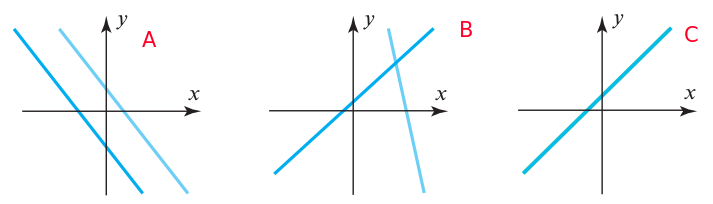
\includegraphics[scale=0.4]{sistema1.png}}\\
    \footnotesize{Fonte:~Anton H, Rorres C. \emph{Elementary Linear Algebra}, 11.\ ed.}
  \end{center}
\end{figure}
\vspace{-0.5cm}
\begin{parts}
  \part \vf[SI] Sistema ``A''
  \part \vf[SPD] Sistema ``B''
  \part \vf[SPI] Sistema ``C''
\end{parts}

\question
A figura abaixo ilustra quatro sistemas de
equações lineares, nos quais \emph{cada sistema é formado por 3
equações}. Indique se o sistema é SPD, SPI ou SI.
\begin{figure}[H]
  \begin{center}
    \fbox{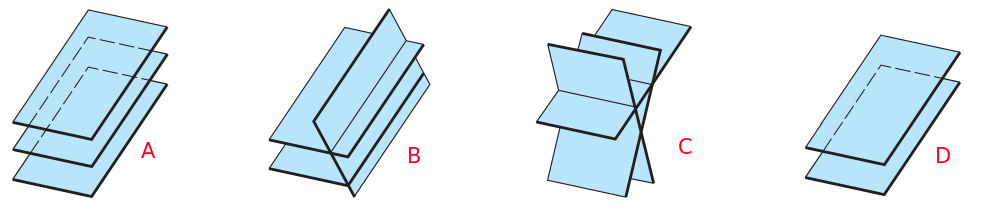
\includegraphics[scale=0.4]{sistema2.png}}\\
    \footnotesize{Fonte:~Anton H, Rorres C. \emph{Elementary Linear Algebra}, 11.\ ed.}
  \end{center}
\end{figure}
\vspace{-0.5cm}
\begin{parts}
  \part \vf[SI] Sistema ``A''
  \part \vf[SI] Sistema ``B''
  \part \vf[SI] Sistema ``C''
  \part \vf[SI] Sistema ``D''
\end{parts}

\question
A figura abaixo ilustra quatro sistemas de
equações lineares, nos quais \emph{cada sistema é formado por 3
equações}. Indique se o sistema é SPD, SPI ou SI.
\begin{figure}[H]
  \begin{center}
    \fbox{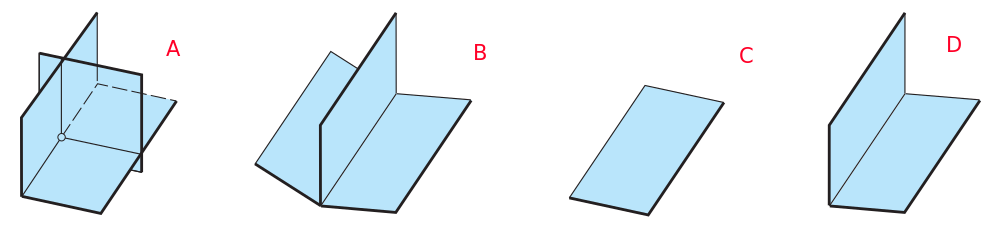
\includegraphics[scale=0.4]{sistema3.png}}\\
    \footnotesize{Fonte:~Anton H, Rorres C. \emph{Elementary Linear Algebra}, 11.\ ed.}
  \end{center}
\end{figure}
\vspace{-0.5cm}
\begin{parts}
  \part \vf[SPD] Sistema ``A''
  \part \vf[SPI] Sistema ``B''
  \part \vf[SPI] Sistema ``C''
  \part \vf[SPI] Sistema ``D''
\end{parts}

\question
Escreva o sistema de equações lineares abaixo: a) na forma da \emph{matriz
aumentada}; e b) na forma da \emph{matriz de coeficientes, variáveis e
termos independentes}.
\begin{center}$A = \begin{cases}
     3x - 5y + 4z - t = 8\\
      y - 2z + 2x     = -3\\
      z - 3t - 2y - x = 1\\
     6t - 5x -  y     = 4 
  \end{cases}$
\end{center}




%%%%%%%%%%%%%%%%%%%%%%%%%%%%%%%%%%%%%%%%%%%%%%%%%%%%%%%%%%%%%%%%%%%%%%%%%%%%%%%%%
%%%%%%%%%%%%%%%%%%%%%%%%%%%%%%%%%%%%%%%%%%%%%%%%%%%%%%%%%%%%%%%%%%%%%%%%%%%%%%%%%
%%%%%%%%%%%%%%%%%%%%%%%%%%%%%%%%%%%%%%%%%%%%%%%%%%%%%%%%%%%%%%%%%%%%%%%%%%%%%%%%%
\fullwidth{\section{Sistemas de Equações Lineares: resolução}}

\question
Resolva o seguinte sistema de equações lineares, pelo método de Cramer:
\begin{center}$A = \begin{cases}
     x + y + 2z = 9\\
    2x + 4y - 3z = 1\\
    3x + 6y - 5z = 0 
  \end{cases}$
\end{center}

\question
Resolva o seguinte sistema de equações lineares, pelo método de Gauss-Jordan:
\begin{center}$B = \begin{cases}
  3x - 3y - 6z =  -3\\
  2x - 2y - 4z = 10\\
  -2x + 3y + z = 7
\end{cases}$
\end{center}

\question
Resolva o seguinte sistema de equações lineares, pelo método de Gauss:
\begin{center}$C = \begin{cases}
    3x - 3y - 6z = -3\\
    2x - 2y - 4z = -2\\
    -2x + 3y + z = 7
  \end{cases}$
\end{center}

\question
Resolva o seguinte sistema de equações lineares, pelo método da matriz inversa:
\begin{center}$D = \begin{cases}
    2x - 4y + 5z = -33\\
    4x - y = -5\\
    -2x + 2y - 3z = 19
  \end{cases}$
\end{center}

\question
Resolva o seguinte sistema de equações lineares, por qualquer método:
\begin{center}$E = \begin{cases}
    x - 2y + 3z = 7\\
    2x + y + z = 4\\
    -3x + 2y - 2z = -10
  \end{cases}$
\end{center}




%%%%%%%%%%%%%%%%%%%%%%%%%%%%%%%%%%%%%%%%%%%%%%%%%%%%%%%%%%%%%%%%%%%%%%%%%%%%%%%%%
%%%%%%%%%%%%%%%%%%%%%%%%%%%%%%%%%%%%%%%%%%%%%%%%%%%%%%%%%%%%%%%%%%%%%%%%%%%%%%%%%
%%%%%%%%%%%%%%%%%%%%%%%%%%%%%%%%%%%%%%%%%%%%%%%%%%%%%%%%%%%%%%%%%%%%%%%%%%%%%%%%%
%\fullwidth{\section{Vetores: conceitos fundamentais}}

%\question
%O que é um vetor? O que diferencia um vetor de um escalar?
%\quatrolinhas

%\question
%A figura abaixo ilustra o \emph{vetor} \vetor{A} juntamente com seus
%\emph{vetores componentes} \vetor{A_x} e \vetor{A_y}.
%\begin{figure}[H]
%  \begin{center}
%%    \fbox{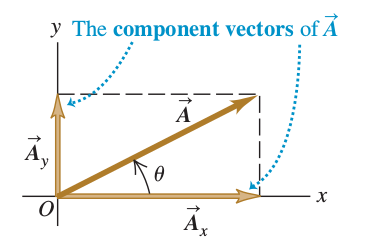
\includegraphics[scale=0.8]{vetor1.png}}\\
%    \footnotesize{Fonte:~Young HD, Freedman RA, Ford
%      LA. \emph{University Physics}, 13.\ ed.}
%  \end{center}
%\end{figure}
%Pergunta-se: qual a diferença/relação entre um determinado vetor e
%seus vetores componentes?
%\quatrolinhas

%%%%%%%%%%%%%%%%%%%%%%%%%%%%%%%%%%%%%%%%%%%%%%%%%%%%%%%%%%%%%%%%%%%%%%%%%%%%%%%%%
%%%%%%%%%%%%%%%%%%%%%%%%%%%%%%%%%%%%%%%%%%%%%%%%%%%%%%%%%%%%%%%%%%%%%%%%%%%%%%%%%
%%%%%%%%%%%%%%%%%%%%%%%%%%%%%%%%%%%%%%%%%%%%%%%%%%%%%%%%%%%%%%%%%%%%%%%%%%%%%%%%%
%%%%%%%%%%%%%%%%%%%%%%%%%%%%%%%%%%%%%%%%%%%%%%%%%%%%%%%%%%%%%%%%%%%%%%%%%%%%%%%%%
%%%%%%%%%%%%%%%%%%%%%%%%%%%%%% TERMINA O DOCUMENTO %%%%%%%%%%%%%%%%%%%%%%%%%%%%%%
%%%%%%%%%%%%%%%%%%%%%%%%%%%%%%%%%%%%%%%%%%%%%%%%%%%%%%%%%%%%%%%%%%%%%%%%%%%%%%%%%
%%%%%%%%%%%%%%%%%%%%%%%%%%%%%%%%%%%%%%%%%%%%%%%%%%%%%%%%%%%%%%%%%%%%%%%%%%%%%%%%%
%%%%%%%%%%%%%%%%%%%%%%%%%%%%%%%%%%%%%%%%%%%%%%%%%%%%%%%%%%%%%%%%%%%%%%%%%%%%%%%%%
%%%%%%%%%%%%%%%%%%%%%%%%%%%%%%%%%%%%%%%%%%%%%%%%%%%%%%%%%%%%%%%%%%%%%%%%%%%%%%%%%
\end{questions}
\end{document}
